\item All the four entries of the $2\times2$ matrix $\vec{P} = \myvec{P_{11} & P_{12}\\ P_{21} & P_{22}}$ are nonzero, and one of its eigenvalues is zero. Which of the following statements is true?
\hfill (EE 2025)
\begin{multicols}{2}
    \begin{enumerate}
        \item $P_{11}P_{22} - P_{12}P_{21} = 1$
        \item $P_{11}P_{22} - P_{12}P_{21} = -1$
        \item $P_{11}P_{22} - P_{12}P_{21} = 0$
        \item $P_{11}P_{22} + P_{12}P_{21} = 0$
    \end{enumerate}
\end{multicols}
%
\item The system of linear equations
\begin{align*}
4x + 2y &= 7 \\
2x + y  &= 6
\end{align*}
has
\hfill (EE 2025)
\begin{multicols}{2}
    \begin{enumerate}
        \item a unique solution
        \item no solution
        \item an infinite number of solutions
        \item exactly two distinct solutions
    \end{enumerate}
\end{multicols}
\item Consider the matrix $\vec{P} = \myvec { 0 & 1 \\ -2 & -3 }$. The value of $e^{\vec{P}}$ is
\hfill (EE 2025)
\begin{multicols}{2}
\begin{enumerate}
    \item $\myvec { 2e^{-2} - 3e^{-1} & e^{-1} - e^{-2} \\ 2e^{-2} - 2e^{-1} & 5e^{-2} - e^{-1}}$
    \item $\myvec { e^{-1} + e^{-2} & 2e^{-2} - e^{-1} \\ 2e^{-1} - 4e^{-2} & 3e^{-1} + e^{-2} }$
    \item $\myvec { 5e^{-2} - 6e^{-1} & 3e^{-1} - e^{-2} \\ 2e^{-2} - 6e^{-1} & 4e^{-2} + e^{-1} }$
    \item $\myvec { 2e^{-1} - e^{-2} & -e^{-1} + 2e^{-2} \\ -2e^{-1} + 2e^{-2} & -e^{-1} + 2e^{-2} }$
\end{enumerate}
\end{multicols}
%
\item A discrete time linear shift-invariant system has an impulse response $h[n]$ with $h[0]=1$, $h[1]=-1$, $h[2]=2$, and zero otherwise. The system is given an input sequence $x[n]$ with $x[0]=x[2]=1$, and zero otherwise. The number of nonzero samples in the output sequence $y[n]$, and the value of $y[2]$ are, respectively
\hfill (EE 2025)
\begin{multicols}{4}
\begin{enumerate}
    \item $5, 2$
    \item $6, 2$
    \item $6, 1$
    \item $5, 3$
\end{enumerate}
\end{multicols}
\item A signal flow graph of a system is given below.
\begin{figure}[H]
	\centering
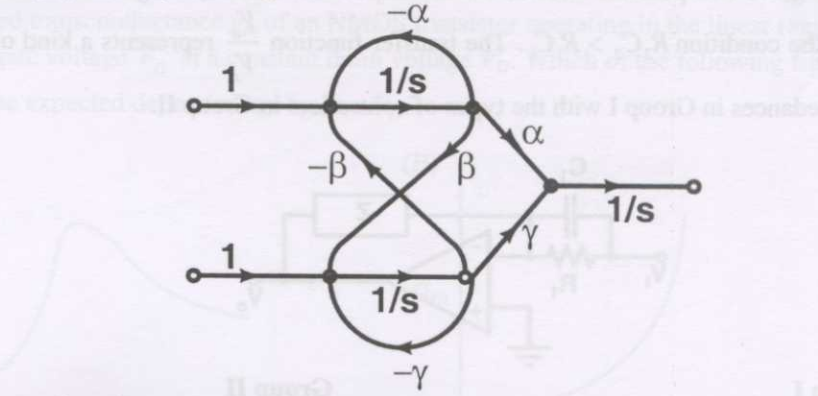
\includegraphics[width=0.5\columnwidth]{GATE/2008/EC/figs/q40.png}
\caption{}
\label{fig:q40}
\end{figure}
The set of equations that correspond to this signal flow graph is
\hfill (EE 2025)
\begin{enumerate}
  \item $\dfrac{d}{dt}
    \myvec {
      x_1 \\ x_2 \\ x_3
    }
    =
    \myvec {
      \beta & -\gamma & 0 \\
      \gamma & \alpha & 0 \\
      -\alpha & -\beta & 0
    }
    \myvec {
      x_1 \\ x_2 \\ x_3
    }
    +
    \myvec {
      1 & 0 \\
      0 & 1 \\
      0 & 0
    }
    \myvec {
      u_1 \\ u_2
    }
   $
  \item $\dfrac{d}{dt}
    \myvec {
      x_1 \\ x_2 \\ x_3
    }
    =
    \myvec {
      0 & \alpha & -\gamma \\
      -\gamma & 0 & \beta \\
      \alpha & \beta & 0
    }
    \myvec {
      x_1 \\ x_2 \\ x_3
    }
    +
    \myvec {
      1 & 0 \\
      0 & 1 \\
      0 & 0
    }
    \myvec {
      u_1 \\ u_2
    }
   $
  \item $\dfrac{d}{dt}
    \myvec {
      x_1 \\ x_2 \\ x_3
    }
    =
    \myvec {
      -\gamma & 0 & \beta \\
      \alpha & \gamma & 0 \\
      -\beta & 0 & -\alpha
    }
    \myvec {
      x_1 \\ x_2 \\ x_3
    }
    +
    \myvec {
      1 & 0 \\
      0 & 1 \\
      0 & 0
    }
    \myvec {
      u_1 \\ u_2
    }
   $
  \item $\dfrac{d}{dt}
    \myvec {
      x_1 \\ x_2 \\ x_3
    }
    =
    \myvec {
      -\gamma & 0 & \beta \\
      0 & \alpha & 0 \\
      -\beta & 0 & -\alpha
    }
    \myvec {
      x_1 \\ x_2 \\ x_3
    }
    +
    \myvec {
      1 & 0 \\
      0 & 1 \\
      0 & 0
    }
    \myvec {
      u_1 \\ u_2
    }
   $
\end{enumerate}
